\section{O Logaritmo Hiperbólico}

Décadas depois da invenção de Napier, em 1647 os logaritmos apareceram em um campo não esperado, na \textbf{área de uma hipérbole}.

Vamos focar o estudo na hipérbole quadrada, isto é, a hipérbole $xy = 1$, ou ainda, $y = \frac{1}{x}$. Queremos estudar a área abaixo do gráfico de $1$ a algum ponto $a$ no eixo $x$. Utilizando linguagem atual do cálculo, queremos estudar:
\[
A(a) = \int_1^a \frac{1}{x} dx
\]

A figura \ref{fig:abaixohiperbole} mostra a área que estamos interessados 

\begin{figure}[H]
    \centering
    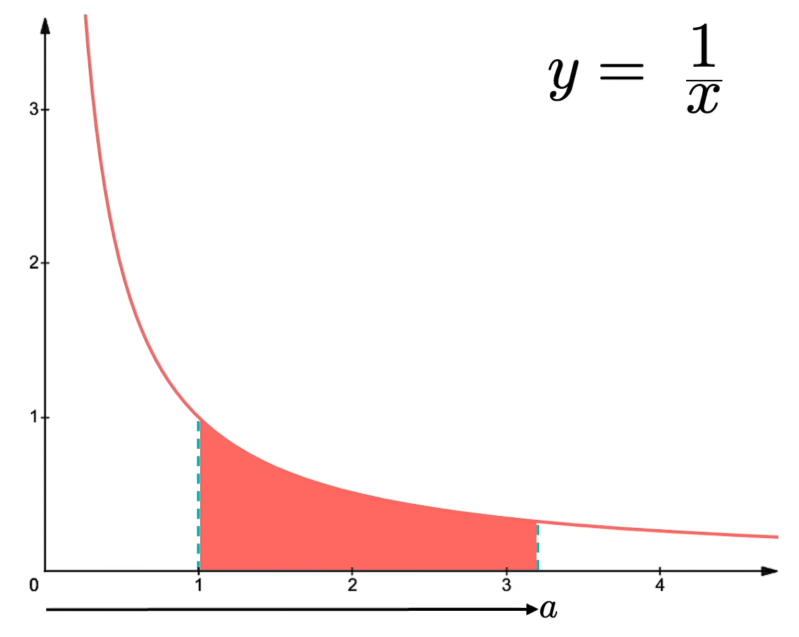
\includegraphics[width=0.5\linewidth]{img/areaabaixohip.png}
    \caption{Área abaixo da Hipérbole de $1$ a $a$}
    \label{fig:abaixohiperbole}
\end{figure}

Calcular essa área se mostrou uma atividade difícil, pois muitos matemáticos tentaram calcular esta área e falharam, entre eles estão Arquimedes, René Descartes e Fermat. Fermat abriu caminho para que o matemático Grégoire de Saint-Vincent (1584 - 1667) finalmente descobrisse a àrea abaixo da hipérbole.

Para calcular essa área, Saint-Vincent a dividiu em retângulos de uma maneira particular, ilustrada na figura \ref{fig:hiperbole}.
O 1° retângulo começa no ponto $a$, o 2° retângulo começa no ponto $ar$, o 3° em $ar^2$ e assim por diante, até chegar em $1$, além disso, note que $r < 1$. A ideia era clara, somar a área de todos os retângulos. Entretanto, não é difícil ver que há um erro com a área real, porém, se $r$ estiver suficientemente próximo de $1$, este erro fica imperceptível.

\begin{figure}[H]
    \centering
    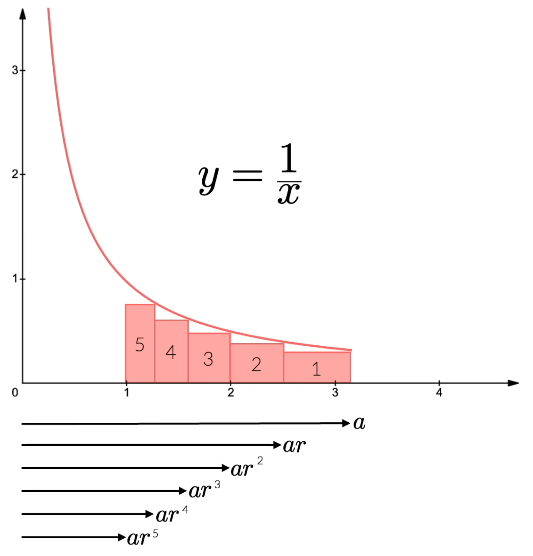
\includegraphics[width=0.5\linewidth]{img/hiperbole.png}
    \caption{Área da Hipérbole via progressão geométrica}
    \label{fig:hiperbole}
\end{figure}

Iremos calcular as áreas destes retângulo para ver se encontramos algo interessante, os resultados estão na tabela \ref{tab:areasvincent}

\begin{table}[h!]
\centering
\begin{tabular}{c c c c}
\toprule
\textbf{Retângulo} & \textbf{Altura} & \textbf{Comprimento} & \textbf{Área} \\
\midrule
1 & $\dfrac{1}{a}$ & $a(1-r)$ & $(1-r)$ \\
\addlinespace
2 & $\dfrac{1}{ar}$ & $ar(1-r)$ & $(1-r)$ \\
\addlinespace
3 & $\dfrac{1}{ar^2}$ & $ar^2(1-r)$ & $(1-r)$ \\
\addlinespace
4 & $\dfrac{1}{ar^3}$ & $ar^3(1-r)$ & $(1-r)$ \\
\addlinespace
5 & $\dfrac{1}{ar^4}$ & $ar^4(1-r)$ & $(1-r)$ \\
\bottomrule
\end{tabular}
\caption{Tabela de Retângulos sob a curva $y=1/x$}
\label{tab:areasvincent}
\end{table}

Encontramos algo interessante! As áreas de cada um desses retângulos são exatamente as mesmas, todas iguais a $(1-r)$. Esse resultado deu Saint-Vincent a seguinte ideia: ele percebeu que isso levava a uma interessante relação entre a distância e a área abaixo da hipérbole, ilustrada na tabela \ref{tab:distarea}.


\begin{table}[h!]
\centering
\begin{tabular}{c c}
\toprule
\textbf{Distância} & \textbf{Área} \\
\midrule
$ar^5$ & $0$ \\
\addlinespace
$ar^4$ & $(1-r)$ \\
\addlinespace
$ar^3$ & $2(1-r)$ \\
\addlinespace
$ar^2$ & $3(1-r)$ \\
\addlinespace
$ar$ & $4(1-r)$ \\
\addlinespace
$a$ & $5(1-r)$ \\
\bottomrule
\end{tabular}
\caption{Relação entre distância e área abaixo da hipérbole}
\label{tab:distarea}
\end{table}

Observe que na distância, de uma linha para outra multiplicamos sempre por $1/r$, enquanto na área somamos sempre $(1-r)$  Isso significa que a distância está seguindo uma progressão geométrica, enquanto a área está seguindo uma progressão aritmética.

Logo, os números na tabela relacionados seguem as mesmas ideias vistas por Napier anos antes. E portanto a relação entre a distância e a área é \textit{logarítmica}.

Daí, Alfonso de Sarasa, um dos estudantes de Saint Vincent, escreveu essa relação de forma explícita, a área da hipérbole até o ponto $a$, foi definida como

\[
A(a) = \log(a)
\]

Esse logaritmo foi chamado de \textbf{logaritmo hiperbólico}. Porém, Saint Vincent e de Sarasa ainda não foram capazes de encontrar uma maneira para calcula-lo. Daí entra uma nova figura: Nicholas Mercator.
